%
% Template Laporan Skripsi/Thesis 
%
% @author  Andreas Febrian, Lia Sadita 
% @version 1.03
%
% Dokumen ini dibuat berdasarkan standar IEEE dalam membuat class untuk 
% LaTeX dan konfigurasi LaTeX yang digunakan Fahrurrozi Rahman ketika 
% membuat laporan skripsi. Konfigurasi yang lama telah disesuaikan dengan 
% aturan penulisan thesis yang dikeluarkan UI pada tahun 2008.
%

%
% Tipe dokumen adalah report dengan satu kolom. 
%
\documentclass[12pt, a4paper, onecolumn, oneside, final]{report}

% Load konfigurasi LaTeX untuk tipe laporan thesis
\usepackage{_internals/uithesis}

% Daftar pemenggalan suku kata dan istilah dalam LaTeX
%
% Hyphenation untuk Indonesia 
%
% @author  Andreas Febrian
% @version 1.00
% 
% Tambahkan cara pemenggalan kata-kata yang salah dipenggal secara otomatis 
% oleh LaTeX. Jika kata tersebut dapat dipenggal dengan benar, maka tidak 
% perlu ditambahkan dalam berkas ini. Tanda pemenggalan kata menggunakan 
% tanda '-'; contoh:
% menarik
%   --> pemenggalan: me-na-rik
%

\hyphenation{
    % alphabhet A
    a-na-li-sa a-tur 
    a-pli-ka-si 
    % alphabhet B
    ba-ngun-an 
    be-be-ra-pa 
    ber-ge-rak
    ber-ke-lan-jut-an 
    ber-pe-nga-ruh 
    % alphabhet C
    ca-ri
    % alphabhet D
    di-sim-pan di-pim-pin de-ngan da-e-rah di-ba-ngun da-pat di-nya-ta-kan 
    di-sim-bol-kan di-pi-lih di-li-hat de-fi-ni-si
    % alphabhet E
    e-ner-gi eks-klu-sif
    % alphabhet F
    fa-si-li-tas
    % alphabhet G
    ga-bung-an ge-rak
    % alphabhet H
    ha-lang-an
    % alphabhet I
    % alphabhet J
    % alphabhet K
    ke-hi-lang-an
    ku-ning 
    kua-li-tas ka-me-ra ke-mung-kin-an ke-se-pa-ham-an
    % alphabhet L
    ling-kung-an
    % alphabhet M
    me-neng-ah
    meng-a-tas-i me-mung-kin-kan me-nge-na-i me-ngi-rim-kan 
    meng-u-bah meng-a-dap-ta-si me-nya-ta-kan mo-di-fi-ka-si
    meng-a-tur
    % alphabhet N
    nya-ta non-eks-klu-sif
    % alphabhet O
    % alphabhet P
	pe-nye-rap-an 
	pe-ngon-trol
    pe-mo-del-an
    pe-ran  pe-ran-an-nya
    pem-ba-ngun-an pre-si-den pe-me-rin-tah prio-ri-tas peng-am-bil-an 
    peng-ga-bung-an pe-nga-was-an pe-ngem-bang-an 
    pe-nga-ruh pa-ra-lel-is-me per-hi-tung-an per-ma-sa-lah-an 
    pen-ca-ri-an peng-struk-tur-an
    % alphabhet Q
    % alphabhet R
    ran-cang-an
    % alphabhet S
    si-mu-la-si sa-ngat
    % alphabhet T
    te-ngah
    ter-da-pat
    % alphabhet U
    % alphabhet V
    % alphabhet W
    % alphabhet X
    % alphabhet Y
    % alphabhet Z
    % special
}

% Load konfigurasi khusus untuk laporan yang sedang dibuat
%-----------------------------------------------------------------------------%
% Informasi Mengenai Dokumen
%-----------------------------------------------------------------------------%
% 
% Judul laporan. 
\var{\judul}{Pengembangan Framework Command and Control Berbasis PowerShell dengan Integrasi Teknik Keystroke Injection menggunakan Rubber Ducky untuk Simulasi Serangan Siber}
% 
% Tulis kembali judul laporan, kali ini akan diubah menjadi huruf kapital
\Var{\Judul}{Pengembangan Framework Command and Control Berbasis PowerShell dengan Integrasi Teknik Keystroke Injection menggunakan Rubber Ducky untuk Simulasi Serangan Siber}
% 
% Tulis kembali judul laporan namun dengan bahasa Ingris
\var{\judulInggris}{Development of a PowerShell-Based Command and Control Framework with Integrated Keystroke Injection Technique Using Rubber Ducky for Cyber Attack Simulation}

% 
% Tipe laporan, dapat berisi Skripsi, Tugas Akhir, Thesis, atau Disertasi
\var{\type}{Skripsi}
% 
% Tulis kembali tipe laporan, kali ini akan diubah menjadi huruf kapital
\Var{\Type}{Skripsi}
% 
% Tulis nama penulis 
\var{\penulis}{Raden Bagus Senopati Kresna Ramdani Galih Rahayu}
% 
% Tulis kembali nama penulis, kali ini akan diubah menjadi huruf kapital
\Var{\Penulis}{Raden Bagus Senopati Kresna Ramdani Galih Rahayu}
% 
% Tulis NPM penulis
\var{\npm}{2106702610}
% 
% Tuliskan Fakultas dimana penulis berada
\Var{\Fakultas}{Teknik}
\var{\fakultas}{Teknik}
% 
% Tuliskan Program Studi yang diambil penulis
\Var{\Program}{Teknik Komputer}
\var{\program}{Teknik Komputer}
% 
% Tuliskan tahun publikasi laporan
\Var{\bulan}{November}
\Var{\tahun}{2024}
% 
% Tuliskan gelar yang akan diperoleh dengan menyerahkan laporan ini
\var{\gelar}{Sarjana Teknik}
% 
% Tuliskan tanggal pengesahan laporan, waktu dimana laporan diserahkan ke 
% penguji/sekretariat
\var{\tanggalPengesahan}{XX Juli 2019} 
% 
% Tuliskan tanggal keputusan sidang dikeluarkan dan penulis dinyatakan 
% lulus/tidak lulus
\var{\tanggalLulus}{XX Juli 2019}
% 
% Tuliskan pembimbing 
\var{\pembimbing}{Prof. Yan Maraden}
% 
% Alias untuk memudahkan alur penulisan paa saat menulis laporan
\var{\saya}{Penulis}

%-----------------------------------------------------------------------------%
% Judul Setiap Bab
%-----------------------------------------------------------------------------%
% 
% Berikut ada judul-judul setiap bab. 
% Silahkan diubah sesuai dengan kebutuhan. 
% 
\Var{\kataPengantar}{Kata Pengantar}
\Var{\babSatu}{Pendahuluan}
\Var{\babDua}{Sekilas Mengenai \latex}
\Var{\babTiga}{Notasi Matematik}
\Var{\babEmpat}{Struktur Berkas}
\Var{\babLima}{Perintah dalam uithesis.sty}
\Var{\babEnam}{Bab Enam}
\Var{\kesimpulan}{Kesimpulan dan Saran}

% Daftar istilah yang mungkin perlu ditandai 
%
% @author  Andreas Febrian
% @version 1.00
% 
% Mendaftar seluruh istilah yang mungkin akan perlu dijadikan 
% italic atau bold pada setiap kemunculannya dalam dokumen. 
% 

\var{\license}{\f{Creative Common License 1.0 Generic}}
\var{\bslash}{$\setminus$}

% Awal bagian penulisan laporan
\begin{document}
%
% Sampul Laporan
%
% Sampul Laporan

%
% @author  unknown
% @version 1.01
% @edit by Andreas Febrian
%

\begin{titlepage}
    \begin{center}    
        \begin{figure}
            \begin{center}
                
\includegraphics[width=2.5cm]{_internals/makara.eps}
            \end{center}
        \end{figure}    
        \vspace*{0cm}
        \bo{
        	UNIVERSITAS INDONESIA\\
        }
        
        \vspace*{1.0cm}
        % judul thesis harus dalam 14pt Times New Roman
        \bo{\Judul} \\[1.0cm]

        \vspace*{2.5 cm}    
        % harus dalam 14pt Times New Roman
        \bo{\Type}

        \vspace*{3 cm}       
        % penulis dan npm
        \bo{\Penulis} \\
        \bo{\npm} \\

        \vspace*{5.0cm}

        % informasi mengenai fakultas dan program studi
        \bo{
        	FAKULTAS \Fakultas\\
        	PROGRAM STUDI \Program \\
        	DEPOK \\
        	\tahun
        }
    \end{center}
\end{titlepage}


%
% Gunakan penomeran romawi
\pagenumbering{roman}

%
% load halaman judul dalam
\addChapter{HALAMAN JUDUL}
%
% Halaman Judul Laporan 
%
% @author  unknown
% @version 1.01
% @edit by Andreas Febrian
%

\begin{titlepage}
    \begin{center}\begin{figure}
            \begin{center}
                
\includegraphics[width=2.5cm]{_internals/makara.eps}
            \end{center}
        \end{figure}    
        \vspace*{0cm}
        \bo{
        	UNIVERSITAS INDONESIA\\
        }
        
        \vspace*{1.0cm}
        % judul thesis harus dalam 14pt Times New Roman
        \bo{\Judul} \\[1.0cm]

        \vspace*{2.5 cm}    
        % harus dalam 14pt Times New Roman
        \bo{\Type} \\
        % keterangan prasyarat
        \bo{Diajukan sebagai salah satu syarat untuk memperoleh gelar \\
        \gelar}\\

        \vspace*{3 cm}       
        % penulis dan npm
        \bo{\Penulis} \\
        \bo{\npm} \\

        \vspace*{5.0cm}

        % informasi mengenai fakultas dan program studi
        \bo{
        	FAKULTAS \Fakultas\\
        	PROGRAM STUDI \Program \\
        	DEPOK \\
        	\bulan\ \tahun
        }
    \end{center}
\end{titlepage}

%
% setelah bagian ini, halaman dihitung sebagai halaman ke 2
\setcounter{page}{2}

%
% load halaman pengesahan
\addChapter{LEMBAR PERSETUJUAN}
%
% Halaman Pengesahan
%
% @author  Andreas Febrian
% @version 1.01
%

\chapter*{HALAMAN PERSETUJUAN}

\vspace*{0.2cm}
\noindent 

\noindent
\begin{tabular}{l l p{11cm}}
	\bo{Judul}&: & \judul \\ 
	\bo{Nama}&: & \penulis \\
	\bo{NPM}&: & \npm \\
\end{tabular} \\

\vspace*{1.2cm}

\noindent Laporan \type~ini telah diperiksa dan disetujui.\\[0.3cm]
\begin{center}
\tanggalPengesahan \\[2cm]


\underline{\pembimbing}\\[0.1cm]
Pembimbing \type
\end{center}

\newpage
%
% load halaman orisinalitas 
\addChapter{LEMBAR PERNYATAAN ORISINALITAS}
%
% Halaman Orisinalitas
%
% @author  Andreas Febrian
% @version 1.01
%

\chapter*{Halaman Pernyataan Orisinalitas}
\vspace*{2cm}

\begin{center}
	\bo{\type~ini adalah hasil karya saya sendiri, \\ 
	dan semua sumber baik yang dikutip maupun dirujuk \\
	telah saya nyatakan dengan benar.} \\
	\vspace*{2.6cm}
	
	\begin{tabular}{l c l}
	\bo{Nama} & : & \bo{\penulis} \\
	\bo{NPM} & : & \bo{\npm} \\ 
	\bo{Tanda Tangan} & : & \\
	& & \\
	& & \\
	\bo{Tanggal} & : & \bo{\tanggalPengesahan} \\	
	\end{tabular}
\end{center}

\newpage
%
%
\addChapter{LEMBAR PENGESAHAN}
%
% Halaman Pengesahan Sidang
%
% @author  Andreas Febrian, Andre Tampubolon 
% @version 1.02
%

\chapter*{HALAMAN PENGESAHAN}

\vspace*{0.4cm}
\noindent 

\noindent
\begin{tabular}{ll p{9cm}}
	\type~ini diajukan oleh&: & \\
	Nama&: & \penulis \\
	NPM&: & \npm \\
	Program Studi&: & \program \\
	Judul \type&: & \judul \\
\end{tabular} \\

\vspace*{1.0cm}

\noindent \bo{Telah berhasil dipertahankan di hadapan Dewan Penguji 
dan diterima sebagai bagian persyaratan yang diperlukan untuk 
memperoleh gelar \gelar~pada Program Studi \program, Fakultas 
\fakultas, Universitas Indonesia.}\\[0.2cm]

\begin{center}
	\bo{DEWAN PENGUJI}
\end{center}

\vspace*{0.3cm}

\begin{tabular}{l l l l }
	& & & \\
	Pembimbing&: & \pembimbing & (\hspace*{3.0cm}) \\
	& & & \\
	Penguji&: & Prof. XXX & (\hspace*{3.0cm}) \\
	& & & \\
	Penguji&: & Prof. XXXX & (\hspace*{3.0cm}) \\
	& & & \\
	Penguji&: & Prof. XXXXXX & (\hspace*{3.0cm}) \\
\end{tabular}\\

\todo{Jangan lupa mengisi nama para penguji.}

\vspace*{2.0cm}

\begin{tabular}{ll l}
	Ditetapkan di&: & Depok\\
	Tanggal&: & \tanggalLulus \\
\end{tabular}


\newpage
%
%
\addChapter{\kataPengantar}
%-----------------------------------------------------------------------------%
\chapter*{Kata Pengantar}
%-----------------------------------------------------------------------------%
Template ini disediakan untuk orang-orang yang berencana menggunakan 
\latex~untuk membuat dokumen tugas akhirnya. 
Mengapa \latex? 
Ada banyak hal mengapa menggunakan \latex, diantaranya:

\begin{enumerate}
	\item \latex~membuat kita jadi lebih fokus terhadap isi dokumen, bukan 
		tampilan atau halaman. 
	\item \latex~memudahkan dalam penulisan persamaan matematis. 
	\item Adanya automatis dalam penomoran caption, bab, subbab, subsubbab, 
		referensi, dan rumus. 
	\item Adanya automatisasi dalam pembuatan daftar isi, daftar gambar, dan
		daftar tabel. 
	\item Adanya kemudahan dalam memberikan referensi dalam tulisan dengan 
		menggunakan label. Cara ini dapat meminimalkan kesalahan pemberian 
		referensi. 
\end{enumerate}

Template ini bebas digunakan dan 
didistribusikan sesuai dengan aturan \license, yang secara sederhana berisi: 

\begin{figure}
	\centering
	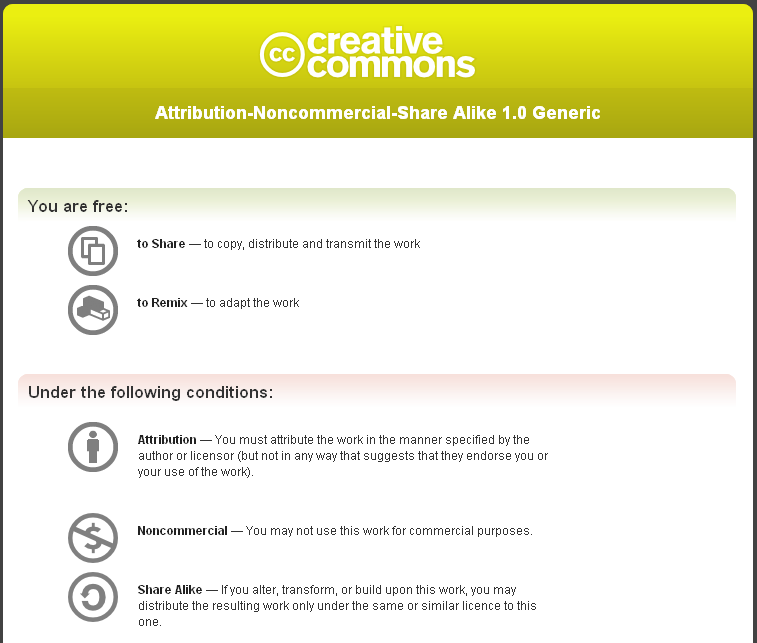
\includegraphics[width=0.74\textwidth]
		{assets/pics/creative_common.png}
	\caption{\license}
	\label{fig:lisensi}
\end{figure}

\pic~\ref{fig:lisensi} diambil dari 
\url{http://creativecommons.org/licenses/by-nc-sa/1.0/deed.en_CA}. 
Jika ingin mengentahui lebih lengkap mengenai \license, silahkan buka 
\url{http://creativecommons.org/licenses/by-nc-sa/1.0/legalcode}. 
Seluruh dokumen yang dibuat dengan menggunakan template ini sepenuhnya 
menjadi hak milik pembuat dokumen dan bebas didistribusikan sesuai dengan 
keperluan masing-masing. 
Lisensi hanya berlaku jika ada orang yang membuat template baru dengan 
menggunakan template ini sebagai dasarnya. 

Dokumen ini dibuat dengan \latex~juga. Untuk meyakinkan Anda, coba lihat 
properti dari dokumen ini dan Anda akan menemukan bagian seperti 
\pic~\ref{fig:pdflatex}. 
Dokumen ini dimaksudkan untuk memberikan gambaran kepada Anda seperti apa 
mudahnya menggunakan \latex~dan juga memperlihatkan betapa bagus dokumen 
yang dihasilkan. 
Seluruh url yang Anda temukan dapat Anda klik. 
Seluruh referensi yang ada juga dapat diklik. 
Untuk mengerti template yang disediakan, Anda tetap harus membuka kode 
\latex~dan bermain-main dengannya. 
Penjelasan dalam PDF ini masih bersifat gambaran dan tidak begitu 
mendetail, dapat dianggap sebagai pengantar singkat. 
Jika Anda merasa kesulitan dengan template ini, mungkin ada baiknya 
Anda belajar sedikit dasar-dasar \latex. 

\begin{figure}
	\centering
	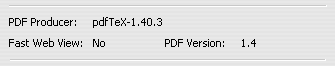
\includegraphics[width=0.54\textwidth]
		{assets/pics/mark.png}
	\caption{Dokumen Dibuat dengan PDFLatex}
	\label{fig:pdflatex}
\end{figure}

Semoga template ini dapat membantu orang-orang yang ingin mencoba menggunakan 
\latex. Semoga template ini juga tidak berhenti disini dengan ada kontribusi 
dari para penggunanya. 
Kami juga ingin berterima kasih kepada Andreas Febrian, Lia Sadita, Fahrurrozi 
Rahman, Andre Tampubolon, dan Erik Dominikus atas kontribusinya dalam template 
ini. 

\vspace*{0.1cm}
\begin{flushright}
Depok, 27 Februari 2019\\[0.1cm]
\vspace*{1cm}
\penulis

\end{flushright}
%
%
\addChapter{LEMBAR PERSETUJUAN PUBLIKASI ILMIAH}
% 
% @author  Andre Tampubolon, Andreas Febrian
% @version 1.01
% 

\chapter*{Halaman Pernyataan Persetujuan Publikasi Tugas Akhir untuk Kepentingan Akademis}

\vspace*{0.2cm}
\noindent 
Sebagai sivitas akademik Universitas Indonesia, saya yang bertanda 
tangan di bawah ini:
\vspace*{0.4cm}


\begin{tabular}{p{4.2cm} l p{6cm}}
	\bo{Nama} & : & \penulis \\ 	
	\bo{NPM} & : & \npm \\
	\bo{Program Studi} & : & \program\\	
	\bo{Fakultas} & : & \fakultas\\
	\bo{Jenis Karya} & : & \type \\
\end{tabular}

\vspace*{0.6cm}
\noindent demi pengembangan ilmu pengetahuan, menyetujui untuk memberikan 
kepada Universitas Indonesia \bo{Hak Bebas Royalti Noneksklusif 
(\textit{Non-exclusive Royalty Free Right})} atas karya ilmiah saya yang berjudul:
\begin{center}
	\judul
\end{center}
beserta perangkat yang ada (jika diperlukan). Dengan Hak Bebas Royalti 
Noneksklusif ini Universitas Indonesia berhak menyimpan, 
mengalihmedia/formatkan, mengelola dalam bentuk pangkalan data 
(\textit{database}), merawat, dan memublikasikan tugas akhir saya selama 
tetap mencantumkan nama saya sebagai penulis/pencipta dan sebagai 
pemilik Hak Cipta. \\

\noindent Demikian pernyatan ini saya buat dengan sebenarnya.

\begin{center}
	\vspace*{0.8cm}
	\begin{tabular}{rl}
		Dibuat di : & Depok \\
		Pada tanggal : & \tanggalPengesahan \\
	\end{tabular}\\

	\vspace*{0.2cm}
	Yang menyatakan \\
	\vspace*{1.1cm}
	(\penulis)
\end{center}

\newpage


%
% 
\addChapter{ABSTRAK}
%
% Halaman Abstrak
%
% @author  Andreas Febrian
% @version 1.00
%

\chapter*{Abstrak}

\vspace*{0.2cm}
{
	\setlength{\parindent}{0pt}
	
	\begin{tabular}{@{}l l p{10cm}}
		Nama&: & \penulis \\
		Program Studi&: & \program \\
		Judul&: & \judul \\
		Pembimbing&: & \pembimbing \\
	\end{tabular}

	\bigskip
	\bigskip

	Tesis ini membahas pengembangan \textit{framework Command and Control} (C2) berbasis \textit{Powershell} dengan integrasi teknik \textit{keystroke injection} yang menggunakan konsep \textit{Rubber Ducky} untuk simulasi serangan siber. Framework ini dirancang untuk mengirimkan perintah otomatis dari server C2 ke perangkat target, sehingga dapat mensimulasikan serangan berbasis injeksi perintah yang realistis dalam pengujian keamanan. Penelitian ini menggunakan pendekatan eksperimental dengan desain deskriptif untuk mengevaluasi efektivitas framework ini dalam menghindari deteksi oleh berbagai sistem keamanan.

	\bigskip

	Kata kunci:\\
	\textit{Command and Control}, \textit{PowerShell}, \textit{Keystroke Injection}, \textit{Rubber Ducky}, Simulasi Serangan Siber, Keamanan Siber
}

\newpage
%
%
%
% Halaman Abstract
%
% @author  Andreas Febrian
% @version 1.00
%

\chapter*{Abstract}

\vspace*{0.2cm}
{
	\setlength{\parindent}{0pt}
	
	\begin{tabular}{@{}l l p{10cm}}
		Name&: & \penulis \\
		Study Program&: & \program \\
		Title&: & \judulInggris \\
		Counsellor&: & \pembimbing \\
	\end{tabular}

	\bigskip
	\bigskip

	The focus of this study is the freshman student of Faculty of Psychology at University of
	Indonesia experience of acquiring, evaluating and using information, when they enroll in
	“Program Dasar Pendidikan Tinggi (PDPT)”. The purpose of this study is to understand
	how freshman students acquire, evaluate and use information. Knowing this will allow
	library to identify changes should be made to improve user education program at
	University of Indonesia. This research is qualitative descriptive interpretive. The data
	were collected by means of deep interview. The researcher suggests that library should
	improve the user education program and provide facilities which can help students to be
	information literate.

	\bigskip

	Key words:\\
	Information literacy, information skills, information
}

\newpage

%
% Daftar isi, gambar, dan tabel
%
\phantomsection
\tableofcontents
\clearpage
\phantomsection
\listoffigures
\clearpage
\phantomsection
\listoftables
\clearpage
\phantomsection
\listoflistings
\clearpage

%
% Gunakan penomeran Arab (1, 2, 3, ...) setelah bagian ini.
%
\pagenumbering{arabic}

%
%
%
%-----------------------------------------------------------------------------%
\chapter{\babSatu}
%-----------------------------------------------------------------------------%
\todo{tambahkan kata-kata pengantar bab 1 disini}


%-----------------------------------------------------------------------------%
\section{Latar Belakang}
%-----------------------------------------------------------------------------%
\todo{tuliskan latar belakang penelitian disini}


%-----------------------------------------------------------------------------%
\section{Permasalahan}
%-----------------------------------------------------------------------------%
Pada bagian ini akan dijelaskan mengenai definisi permasalahan 
yang \saya~hadapi dan ingin diselesaikan serta asumsi dan batasan 
yang digunakan dalam menyelesaikannya.


%-----------------------------------------------------------------------------%
\subsection{Definisi Permasalahan}
%-----------------------------------------------------------------------------%
\todo{Tuliskan permasalahan yang ingin diselesaikan. Bisa juga
	berbentuk pertanyaan}


%-----------------------------------------------------------------------------%
\subsection{Batasan Permasalahan}
%-----------------------------------------------------------------------------%
\todo{Umumnya ada asumsi atau batasan yang digunakan untuk 
	menjawab pertanyaan-pertanyaan penelitian diatas.}


%-----------------------------------------------------------------------------%
\section{Tujuan}
%-----------------------------------------------------------------------------%
\todo{Tuliskan tujuan penelitian.}


%-----------------------------------------------------------------------------%
\section{Posisi Penelitian}
%-----------------------------------------------------------------------------%
\todo{Posisi penelitian Anda jika dilihat secara bersamaan dengan 
	peneliti-peneliti lainnya. Akan lebih baik lagi jika ikut menyertakan 
	diagram yang menjelaskan hubungan dan keterkaitan antar 
	penelitian-penelitian sebelumnya}


%-----------------------------------------------------------------------------%
\section{Metodologi Penelitian}
%-----------------------------------------------------------------------------%
\todo{Tuliskan metodologi penelitian yang digunakan.}


%-----------------------------------------------------------------------------%
\section{Sistematika Penulisan}
%-----------------------------------------------------------------------------%
Sistematika penulisan laporan adalah sebagai berikut:
\begin{itemize}
	\item Bab 1 \babSatu \\
	\item Bab 2 \babDua \\
	\item Bab 3 \babTiga \\
	\item Bab 4 \babEmpat \\
	\item Bab 5 \babLima \\
	\item Bab 6 \babEnam \\
	\item Bab 7 \kesimpulan \\
\end{itemize}

\todo{Tambahkan penjelasan singkat mengenai isi masing-masing bab.}


%-----------------------------------------------------------------------------%
\chapter{\babDua}
%-----------------------------------------------------------------------------%
\todo{tambahkan kata-kata pengantar bab 2 disini}

%-----------------------------------------------------------------------------%
\section{Command and Control (C2) Framework}
%-----------------------------------------------------------------------------%
Command and Control (C2) adalah komponen utama dalam ekosistem serangan siber yang memungkinkan peretas mengendalikan perangkat yang telah disusupi. Framework C2 dirancang untuk mengelola komunikasi antara perangkat target (client) dan server pengendali (C2 server). Dalam serangan siber, framework ini digunakan untuk mengirimkan perintah, menerima data, atau bahkan menjalankan skrip secara jarak jauh.


Framework C2 berbasis PowerShell menawarkan berbagai keuntungan, seperti fleksibilitas, kompatibilitas tinggi dengan sistem Windows, dan kemampuannya untuk menyamarkan aktivitas berbahaya. PowerShell sering dimanfaatkan karena sifatnya yang merupakan komponen bawaan Windows, sehingga meminimalkan risiko terdeteksi oleh sistem keamanan.


Framework Command and Control (C2) berperan sebagai inti dalam pengembangan penelitian ini, di mana framework ini digunakan untuk mengelola komunikasi antara server dan perangkat target. Framework berbasis PowerShell dipilih karena fleksibilitas dan kompatibilitasnya dengan sistem operasi Windows, yang merupakan sistem operasi yang sering menjadi target serangan. Dalam penelitian ini, framework C2 dikembangkan untuk mendukung pengiriman perintah dan menerima data hasil serangan melalui simulasi serangan siber. 

%-----------------------------------------------------------------------------%
\section{Keystroke Injection}
%-----------------------------------------------------------------------------%
Keystroke injection adalah metode untuk mensimulasikan input keyboard pada perangkat target secara otomatis. Teknik ini sering digunakan oleh peretas untuk menyisipkan perintah atau payload secara langsung ke perangkat korban tanpa memerlukan interaksi pengguna.


Dalam penelitian ini, Digispark digunakan sebagai perangkat untuk keystroke injection. Digispark adalah mikrokontroler berbasis ATtiny85 yang dapat diprogram melalui Arduino IDE. Dengan menggunakan library DigiKeyboard.h, Digispark mampu berfungsi sebagai keyboard USB dan mengirimkan input berupa keystroke ke perangkat target. Teknik ini sangat efektif karena perangkat target menganggap Digispark sebagai perangkat input yang sah.

Teknik keystroke injection dikaitkan langsung dengan metode pengiriman payload ke perangkat korban. Penulis menggunakan teknik ini karena kemampuannya untuk menyisipkan perintah secara langsung ke sistem target melalui input keyboard yang disimulasikan. Teknik ini relevan untuk mendukung penelitian karena memungkinkan serangan dilakukan dengan waktu singkat tanpa memerlukan instalasi perangkat lunak tambahan pada perangkat korban, sehingga meningkatkan efisiensi simulasi serangan. 

%-----------------------------------------------------------------------------%
\section{Powershell}
%-----------------------------------------------------------------------------%
PowerShell adalah shell perintah dan bahasa pemrograman yang dirancang untuk otomatisasi tugas dan konfigurasi sistem, khususnya pada sistem operasi Windows. Dalam konteks keamanan siber, PowerShell sering dimanfaatkan untuk berbagai aktivitas, seperti pengumpulan informasi, eksekusi skrip jarak jauh, dan manipulasi data.


PowerShell memiliki beberapa keunggulan dalam pengembangan framework C2, antara lain:
\begin{itemize}
    \item Kemampuan scripting yang kuat untuk membuat payload kompleks.
    \item Akses langsung ke API Windows, memungkinkan pengendalian sistem operasi.
    \item Kompatibilitas bawaan dengan sebagian besar sistem Windows, mengurangi kebutuhan untuk instalasi tambahan. 
\end{itemize}


PowerShell dipilih sebagai bahasa pemrograman utama untuk mengembangkan framework Command and Control karena sifatnya yang kuat dalam scripting dan mendukung akses langsung ke API Windows. Dalam penelitian ini, PowerShell digunakan untuk membuat payload yang disisipkan ke perangkat target melalui keystroke injection, serta untuk berkomunikasi dengan server C2 untuk mengirimkan data atau menjalankan perintah. Pemanfaatan PowerShell memungkinkan simulasi serangan yang lebih realistis dan efektif. 
%-----------------------------------------------------------------------------%
\section{Digispark}
%-----------------------------------------------------------------------------%
Digispark adalah mikrokontroler kecil berbasis ATtiny85 yang sering digunakan dalam berbagai proyek elektronik. Ukurannya yang kecil, biaya yang terjangkau, dan kompatibilitas dengan Arduino IDE menjadikan Digispark pilihan populer dalam teknik keystroke injection.


Library \verb|DigiKeyboard.h| memungkinkan Digispark untuk bertindak sebagai perangkat input USB yang mensimulasikan keyboard. Dalam penelitian ini, Digispark diprogram untuk mengirimkan perintah PowerShell ke perangkat target melalui simulasi input keyboard. Keunggulan Digispark adalah kemampuannya untuk menjalankan tugas ini dengan cepat dan tanpa perlu modifikasi besar pada perangkat target.

 
Penulis menggunakan mikrokontroler Digispark karena perangkat keras ini memiliki library \verb|DigiKeyboard.h| yang memungkinkan penulis untuk melakukan simulasi keystroke injection pada perangkat korban. Digispark dipilih karena ukurannya yang kecil, biaya yang rendah, dan kompatibilitas dengan Arduino IDE, sehingga mempermudah pengembangan perangkat untuk menyisipkan perintah PowerShell ke perangkat target. Dalam penelitian ini, Digispark menjadi komponen penting untuk mengintegrasikan perangkat keras dengan framework C2. 

%-----------------------------------------------------------------------------%
\section{Amazon AWS}
%-----------------------------------------------------------------------------%
Amazon Web Services (AWS) adalah platform cloud yang menyediakan berbagai layanan, termasuk server yang dapat digunakan sebagai pusat Command and Control (C2). Dalam penelitian ini, AWS digunakan untuk: 
\begin{itemize}
    \item Menyediakan server yang dapat menerima dan mengolah data dari perangkat target.
    \item Mendukung komunikasi aman antara perangkat target dan server melalui protokol HTTPS.
    \item Mengelola penyimpanan data hasil serangan untuk analisis lebih lanjut. 
\end{itemize}
 

AWS digunakan sebagai server Command and Control karena kemampuannya menyediakan infrastruktur yang skalabel dan aman untuk mendukung penelitian. Server AWS berfungsi sebagai pusat kendali untuk menerima data dari perangkat korban dan mengirimkan perintah selama simulasi serangan. Korelasinya dengan penelitian adalah memberikan fleksibilitas dalam pengelolaan server C2, serta mendukung pengujian berbagai skenario serangan dengan komunikasi aman melalui protokol HTTPS. 
%-----------------------------------------------------------------------------%

%-----------------------------------------------------------------------------%
\chapter{\babTiga}
%-----------------------------------------------------------------------------%
Bab ini akan menjelaskan perancangan sistem dan model framework dari Sistem Serangan menggunakan Digispark berbasis Keystroke Injection


%-----------------------------------------------------------------------------%
\section{Alur Penelitian}
%-----------------------------------------------------------------------------%

\begin{figure}
	\centering
	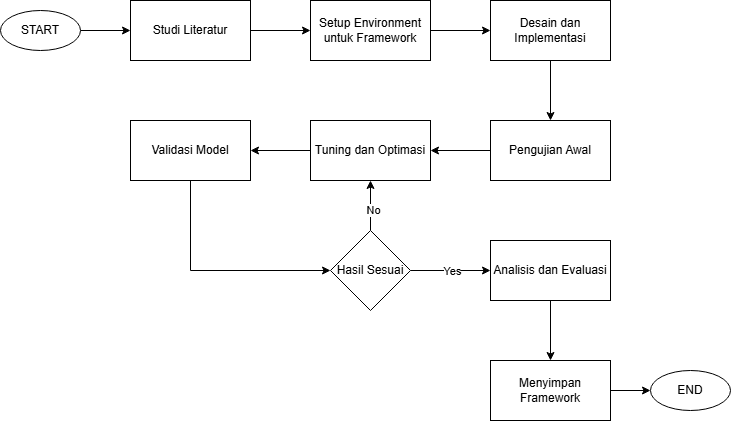
\includegraphics[width=0.95\textwidth]
		{assets/pics/Alur Penelitian.png}
	\caption{Diagram Alur Penelitian}
	\label{fig:testGambar}
\end{figure}

Alur penelitian ini dimulai dengan studi literatur, di mana peneliti mengumpulkan referensi terkait konsep Command and Control (C2), PowerShell, keystroke injection, dan perangkat Digispark. Setelah itu, dilakukan setup environment untuk framework, termasuk pengaturan server C2, perangkat korban, dan perangkat Digispark sebagai media keystroke injection.


Langkah berikutnya adalah desain dan implementasi, yang mencakup perancangan komponen framework serta pengintegrasian modul PowerShell dan Digispark. Setelah framework selesai dikembangkan, dilakukan pengujian awal untuk mengevaluasi performanya dalam skenario simulasi serangan. Jika hasil pengujian tidak sesuai dengan ekspektasi, penelitian dilanjutkan dengan tuning dan optimasi, di mana parameter framework diperbaiki dan diuji ulang hingga mendapatkan hasil yang diinginkan.


Setelah hasil sesuai, framework dievaluasi secara menyeluruh dalam tahap analisis dan evaluasi, untuk memastikan efektivitas dan fungsionalitasnya. Penelitian diakhiri dengan menyimpan framework dalam bentuk final yang siap untuk digunakan dan didokumentasikan.

%-----------------------------------------------------------------------------%
\section{Setup Environment}
%-----------------------------------------------------------------------------%
Dengan tujuan simulasi serangan siber yang realistis, penulis menggunakan perangkat keras berikut:
\begin{itemize}
    \item CPU   : 13th Gen Intel(R) Core(TM) i5-13500H   2.60 GHz
    \item RAM   : 16.0 GB (15.7 GB usable)
    \item Digispark Rev.3

\end{itemize}

Penulis menggunakan perangkat lunak sebagai berikut:
\begin{itemize}
    \item OS    : Windows 11 (version 22631.4602)
    \item Arduino IDE
    \item Duckuino
    \item Amazone AWS

\end{itemize}


%-----------------------------------------------------------------------------%
\section{Implementasi Framework}
%-----------------------------------------------------------------------------%
Implementasi framework dilakukan dengan beberapa tahapan penting yang saling berkaitan. Tahap pertama adalah pemrograman perangkat Digispark menggunakan Arduino IDE. Dalam proses ini, library DigiKeyboard.h dimanfaatkan untuk memungkinkan Digispark mensimulasikan input keyboard secara otomatis. Script yang diprogram pada Digispark berisi instruksi untuk menyisipkan payload PowerShell ke dalam perangkat target. Payload ini dirancang untuk dapat dieksekusi secara otomatis begitu Digispark tersambung ke perangkat target, sehingga pengguna tidak memerlukan intervensi tambahan.


Tahap kedua adalah pengembangan script PowerShell sebagai bagian dari agen untuk server Command and Control (C2). Script ini dirancang untuk menjalankan fungsi-fungsi penting, seperti mengumpulkan data dari perangkat target, mengirimkan data tersebut ke server C2 yang telah dikonfigurasi di Amazon AWS, serta mengeksekusi perintah yang dikirimkan dari server. Dalam pengembangannya, dilakukan berbagai penyesuaian untuk memastikan kompatibilitas script dengan sistem operasi Windows 11, yang menjadi platform target penelitian ini.


Tahap terakhir adalah integrasi seluruh komponen framework. Dalam tahap ini, Digispark, script payload PowerShell, dan server C2 disatukan dalam sebuah alur kerja yang terkoordinasi. Proses integrasi ini bertujuan untuk memastikan bahwa setiap komponen dapat saling berkomunikasi secara efisien dan mendukung simulasi serangan siber yang telah dirancang. Hasil dari implementasi ini diharapkan dapat menghasilkan framework yang tidak hanya fungsional, tetapi juga fleksibel dalam mensimulasikan berbagai skenario serangan.

%-----------------------------------------------------------------------------%
\section{Pengujian Awal}
Setelah implementasi framework selesai, pengujian awal dilakukan untuk memastikan bahwa setiap komponen bekerja sesuai dengan desain yang direncanakan. Pada tahap ini, simulasi serangan dimulai dengan menggunakan Digispark untuk menyisipkan payload PowerShell ke perangkat target. Setelah payload dieksekusi, perangkat target diharapkan dapat terhubung ke server C2 melalui koneksi yang telah dikonfigurasi.


Hasil dari pengujian awal menunjukkan adanya kendala pada proses komunikasi antara perangkat target dan server C2. Script payload yang dijalankan pada perangkat target tidak berhasil mengirimkan data ke server C2 sebagaimana yang diharapkan. Masalah ini dapat disebabkan oleh beberapa faktor, seperti kesalahan dalam konfigurasi server, ketidaksesuaian format data, atau adanya pembatasan sistem pada perangkat target.


Kendala ini memberikan indikasi bahwa framework memerlukan penyesuaian lebih lanjut untuk memastikan keberhasilan komunikasi antara perangkat target dan server C2. Hasil pengujian awal ini menjadi dasar untuk melakukan tuning dan optimasi pada tahap berikutnya, dengan fokus pada perbaikan script payload, pengaturan ulang server C2, dan peningkatan mekanisme injeksi keystroke pada Digispark.
%-----------------------------------------------------------------------------%

%-----------------------------------------------------------------------------%
\section{Tuning dan Optimasi}
Setelah menemukan kendala pada pengujian awal, proses tuning dan optimasi dilakukan untuk meningkatkan performa framework yang telah dikembangkan. Langkah pertama adalah meninjau kembali script payload PowerShell yang digunakan untuk memastikan bahwa perintah-perintah yang dieksekusi sesuai dengan kebutuhan. Penyesuaian dilakukan pada struktur script, termasuk mekanisme pengiriman data ke server C2. Dalam hal ini, penambahan logging pada script PowerShell membantu dalam mengidentifikasi titik-titik kegagalan selama proses komunikasi berlangsung.


Langkah berikutnya adalah memperbaiki konfigurasi server C2 yang dihosting di Amazon AWS. Proses ini melibatkan pengaturan ulang firewall dan port yang digunakan untuk komunikasi dengan perangkat target. Selain itu, dilakukan verifikasi terhadap parameter protokol yang digunakan, seperti protokol HTTP atau HTTPS, untuk memastikan bahwa koneksi dapat diterima dan diproses oleh server C2 tanpa hambatan.


Perangkat Digispark juga mendapat perhatian dalam proses optimasi ini. Script yang diunggah ke perangkat diperbarui untuk memperbaiki timing eksekusi keystroke, memastikan bahwa payload berhasil dimasukkan ke perangkat target tanpa terdeteksi oleh mekanisme keamanan sistem operasi. Percobaan berulang dilakukan untuk menyempurnakan urutan perintah dan waktu jeda antar-eksekusi agar proses injeksi dapat berjalan lebih cepat dan akurat.


Tahapan tuning dan optimasi ini dilanjutkan dengan simulasi serangan menggunakan framework yang telah diperbarui. Setiap perubahan dievaluasi berdasarkan keberhasilan komunikasi antara perangkat target dan server C2, serta efisiensi injeksi payload oleh Digispark. Hasil dari tahapan ini menunjukkan perbaikan signifikan dalam performa framework, di mana koneksi ke server C2 berhasil dijalin, dan payload dapat dieksekusi dengan baik di perangkat target. Proses tuning dan optimasi ini menjadi kunci untuk memastikan framework dapat digunakan secara efektif dalam mensimulasikan serangan siber yang realistis.
%-----------------------------------------------------------------------------%
%-----------------------------------------------------------------------------%
\chapter{\babEmpat}
%-----------------------------------------------------------------------------%
\todo{tambahkan kata-kata pengantar bab 1 disini}

%-----------------------------------------------------------------------------%
\section{thesis.tex}
%-----------------------------------------------------------------------------%
Berkas ini berisi seluruh berkas Latex yang dibaca, jadi bisa dikatakan sebagai 
berkas utama. Dari berkas ini kita dapat mengatur bab apa saja yang ingin 
kita tampilkan dalam dokumen.


%-----------------------------------------------------------------------------%
\section{laporan\_setting.tex}
%-----------------------------------------------------------------------------%
Berkas ini berguna untuk mempermudah pembuatan beberapa template standar. 
Anda diminta untuk menuliskan judul laporan, nama, npm, dan hal-hal lain yang 
dibutuhkan untuk pembuatan template. 


%-----------------------------------------------------------------------------%
\section{istilah.tex}
%-----------------------------------------------------------------------------%
Berkas istilah digunakan untuk mencatat istilah-istilah yang digunakan. 
Fungsinya hanya untuk memudahkan penulisan.
Pada beberapa kasus, ada kata-kata yang harus selalu muncul dengan tercetak 
miring atau tercetak tebal. 
Dengan menjadikan kata-kata tersebut sebagai sebuah perintah \latex~tentu akan 
mempercepat dan mempermudah pengerjaan laporan. 


%-----------------------------------------------------------------------------%
\section{hype.indonesia.tex}
%-----------------------------------------------------------------------------%
Berkas ini berisi cara pemenggalan beberapa kata dalam bahasa Indonesia. 
\latex~memiliki algoritma untuk memenggal kata-kata sendiri, namun untuk 
beberapa kasus algoritma ini memenggal dengan cara yang salah. 
Untuk memperbaiki pemenggalan yang salah inilah cara pemenggalan yang benar 
ditulis dalam berkas hype.indonesia.tex.


%-----------------------------------------------------------------------------%
\section{pustaka.tex}
%-----------------------------------------------------------------------------%
Berkas pustaka.tex berisi seluruh daftar referensi yang digunakan dalam 
laporan. 
Anda bisa membuat model daftar referensi lain dengan menggunakan bibtex.
Untuk mempelajari bibtex lebih lanjut, silahkan buka 
\url{http://www.bibtex.org/Format}. 
Untuk merujuk pada salah satu referensi yang ada, gunakan perintah \bslash 
cite, e.g. \bslash cite\{lankton2008introduction\} yang akan akan memunculkan 
\cite{lankton2008introduction}


%-----------------------------------------------------------------------------%
\section{bab[1 - 6].tex}
%-----------------------------------------------------------------------------%
Berkas ini berisi isi laporan yang Anda tulis. 
Setiap nama berkas e.g. bab1.tex merepresentasikan bab dimana tulisan tersebut 
akan muncul. 
Sebagai contoh, kode dimana tulisan ini dibaut berada dalam berkas dengan nama 
bab4.tex. 
Ada enam buah berkas yang telah disiapkan untuk mengakomodir enam bab dari 
laporan Anda, diluar bab kesimpulan dan saran. 
Jika Anda tidak membutuhkan sebanyak itu, silahkan hapus kode dalam berkas 
thesis.tex yang memasukan berkas \latex~yang tidak dibutuhkan;  contohnya 
perintah \bslash include\{bab6.tex\} merupakan kode untuk memasukan berkas 
bab6.tex kedalam laporan.

%-----------------------------------------------------------------------------%
\section{Penulisan \textit{code} atau \textit{pseudocode} program}
%-----------------------------------------------------------------------------%

\subsection{\textit{Inline}}

Dengan perintah \verb|\verb|: \verb|System.out.println("Hello, World");| \\
Dengan perintah \textit{custom} \verb|\code|: \code{System.out.println("Hello, World"); }
Dengan perintah \verb|\mintinline|: \mintinline{java}{System.out.println("Hello, World"); }

\subsection{\textit{Multiline}}

Dengan perintah \verb|verbatim|: 

\begin{verbatim}	
public class HelloWorld {
    public static void main(String[] args) {
        // Prints "Hello, World" to the terminal window.
        System.out.println("Hello, World");
    }
}
\end{verbatim}

Dengan perintah \verb|minted|: Kode \ref{code:hw:minted}
\begin{listing}[H]
    \begin{minted}{python}
def binary_accuracy(y_true, y_pred):
    return K.mean(K.equal(y_true, K.round(y_pred)), axis=-1)


def categorical_accuracy(y_true, y_pred):
    return K.cast(K.equal(K.argmax(y_true, axis=-1),
                          K.argmax(y_pred, axis=-1)),
                  K.floatx())


def sparse_categorical_accuracy(y_true, y_pred):
    # reshape in case it's in shape (num_samples, 1) instead of (num_samples,)
    if K.ndim(y_true) == K.ndim(y_pred):
        y_true = K.squeeze(y_true, -1)
    # convert dense predictions to labels
    y_pred_labels = K.argmax(y_pred, axis=-1)
    y_pred_labels = K.cast(y_pred_labels, K.floatx())
    return K.cast(K.equal(y_true, y_pred_labels), K.floatx())


def top_k_categorical_accuracy(y_true, y_pred, k=5):
    return K.mean(K.in_top_k(y_pred, K.argmax(y_true, axis=-1), k), axis=-1)


def sparse_top_k_categorical_accuracy(y_true, y_pred, k=5):
    # If the shape of y_true is (num_samples, 1), flatten to (num_samples,)
    return K.mean(K.in_top_k(y_pred, K.cast(K.flatten(y_true), 'int32'), k),
                  axis=-1)
    \end{minted}
    \caption{An excerpt from keras: \url{https://github.com/keras-team/keras/blob/master/keras/metrics.py}}
    \label{code:hw:minted}
\end{listing}

Konfigurasi tampilan bisa dilakukan di \verb|uithesis.sty| dengan referensi dokumentasi di \url{https://github.com/gpoore/minted/blob/master/source/minted.pdf}
%-----------------------------------------------------------------------------%
\chapter{\babLima}
%-----------------------------------------------------------------------------%
\todo{Tambahkan kata-kata pengantar bab 5 disini.}


%-----------------------------------------------------------------------------%
\section{Mengubah Tampilan Teks}
%-----------------------------------------------------------------------------%
Beberapa perintah yang dapat digunakan untuk mengubah tampilan adalah: 
\begin{itemize}
	\item \bslash f \\
		Merupakan alias untuk perintah \bslash textit, contoh 
		\f{contoh hasil tulisan}.
	\item \bslash bi \\
		\bi{Contoh hasil tulisan}.
	\item \bslash bo \\
		\bo{Contoh hasil tulisan}.
	\item \bslash m \\
		Contoh\ hasil\ tulisan: $\alpha \not= \m{\alpha}$
	\item \bslash code \\ 
		\code{Contoh hasil tulisan}.
\end{itemize}


%-----------------------------------------------------------------------------%
\section{Memberikan Catatan}
%-----------------------------------------------------------------------------%
Ada dua perintah untuk memberikan catatan penulisan dalam dokumen yang Anda 
kerjakan, yaitu: 
\begin{itemize}
	\item \bslash todo \\
		Contoh: \\ \todo{Contoh bentuk todo.}
	\item \bslash todoCite \\ 
		Contoh: \todoCite
\end{itemize}


%-----------------------------------------------------------------------------%
\section{Menambah Isi Daftar Isi}
%-----------------------------------------------------------------------------%
Terkadang ada kebutuhan untuk memasukan kata-kata tertentu kedalam Daftar Isi. 
Perintah \bslash addChapter dapat digunakan untuk judul bab dalam Daftar isi. 
Contohnya dapat dilihat pada berkas thesis.tex.


%-----------------------------------------------------------------------------%
\section{Memasukan PDF}
%-----------------------------------------------------------------------------%
Untuk memasukan PDF dapat menggunakan perintah \bslash inpdf yang menerima satu 
buah argumen. Argumen ini berisi nama berkas yang akan digabungkan dalam 
laporan. PDF yang dimasukan degnan cara ini akan memiliki header dan footer 
seperti pada halaman lainnya. 

\inpdf{assets/pdfs/include}

Cara lain untuk memasukan PDF adalah dengan menggunakan perintah \bslash putpdf 
dengan satu argumen yang berisi nama berkas pdf. Berbeda dengan perintah 
sebelumnya, PDF yang dimasukan dengan cara ini tidak akan memiliki footer atau 
header seperti pada halaman lainnya. 

\putpdf{assets/pdfs/include}


%-----------------------------------------------------------------------------%
\section{Membuat Perintah Baru}
%-----------------------------------------------------------------------------%
Ada dua perintah yang dapat digunakan untuk membuat perintah baru, yaitu: 
\begin{itemize}
	\item \bslash Var \\
		Digunakan untuk membuat perintah baru, namun setiap kata yang diberikan
		akan diproses dahulu menjadi huruf kapital. 
		Contoh jika perintahnya adalah \bslash Var\{adalah\} makan ketika 
		perintah \bslash Var dipanggil, yang akan muncul adalah ADALAH. 
	\item \bslash var \\
		Digunakan untuk membuat perintah atau baru. 
\end{itemize}


%-----------------------------------------------------------------------------%
\chapter{\babEnam}
%-----------------------------------------------------------------------------%
\todo{tambahkan kata-kata pengantar bab 6 disini}


%---------------------------------------------------------------
\chapter{\kesimpulan}
%---------------------------------------------------------------
\todo{Tambahkan kesimpulan dan saran terkait dengan perkerjaan 
	yang dilakukan.}


%---------------------------------------------------------------
\section{Kesimpulan}
%---------------------------------------------------------------


%---------------------------------------------------------------
\section{Saran}
%---------------------------------------------------------------


%
% Daftar Pustaka
%\input{pustaka}

% Alternatif manajemen daftar pustaka dengan \bibliography
\bibliographystyle{apalike}
\bibliography{pustaka}

%
% Lampiran 
%
% \begin{appendix}
% 	%
% @author  Andreas Febrian
% @version 1.00 
% 
% Hanya sebuah pembatas bertuliskan LAMPIRAN ditengah halaman. 
% 

\begin{titlepage}
	\centering 
	\vspace*{6cm}
	\noindent \Huge{LAMPIRAN}
	\addChapter{LAMPIRAN}
\end{titlepage}
% 	\setcounter{page}{2}\textbf{}
% 	%-----------------------------------------------------------------------------%
\addChapter{Lampiran 1}
\chapter*{Lampiran 1}
%-----------------------------------------------------------------------------%
% \end{appendix}

\end{document}